\documentclass[11pt,a4paper]{article}
\usepackage[margin=2cm]{geometry}
\usepackage[T1]{fontenc}
\usepackage[utf8]{inputenc}
\usepackage{lmodern,microtype}
\usepackage{amsmath,amssymb,mathtools,bm}
\usepackage{booktabs,tabularx,array}
\usepackage{graphicx,float,caption}
\usepackage{xcolor,hyperref,fancyhdr,titlesec,enumitem}
\usepackage[most]{tcolorbox}
\usepackage{tikz}
\usetikzlibrary{arrows.meta,positioning,fit,calc}
\definecolor{deepblue}{RGB}{28,63,105}
\definecolor{deepgreen}{RGB}{38,105,79}
\definecolor{deeporange}{RGB}{170,92,20}
\definecolor{softblue}{RGB}{232,241,250}
\definecolor{softgreen}{RGB}{235,247,240}
\definecolor{softorange}{RGB}{253,243,226}
\hypersetup{colorlinks=true,linkcolor=deepblue,urlcolor=deeporange,pdftitle={Geometry-MMALS G1 v1.1.2 Specification},pdfauthor={Guillaume Harbonnier}}
\pagestyle{fancy}\fancyhf{}\lhead{Geometry-MMALS G1}\rhead{v1.1.2 specification}\cfoot{\thepage}\setlength{\headheight}{14pt}
\titleformat{\section}{\Large\bfseries\color{deepblue}}{\thesection}{0.8em}{}
\titleformat{\subsection}{\large\bfseries\color{deepgreen}}{\thesubsection}{0.8em}{}
\newtcolorbox{decisionbox}[1][]{title={#1},colback=softorange,colframe=deeporange!55,boxrule=.6pt,arc=2pt}
\newtcolorbox{designbox}[1][]{title={#1},colback=softblue,colframe=deepblue!45,boxrule=.6pt,arc=2pt}
\newtcolorbox{claimbox}[1][]{title={#1},colback=softgreen,colframe=deepgreen!45,boxrule=.6pt,arc=2pt}
\newcommand{\R}{\mathbb R}\newcommand{\E}{\mathbb E}\newcommand{\loss}{\mathcal L}\newcommand{\norm}[1]{\left\lVert #1\right\rVert}
\begin{document}
\begin{titlepage}\centering
\vspace*{0.8cm}{\Huge\bfseries\color{deepblue} Geometry-MMALS G1 v1.1.2\par}
\vspace{0.3cm}{\LARGE Smooth Simplex-Residual Routing\par}
\vspace{0.1cm}{\LARGE and Covariance-Aware Context Diagnostics\par}
\vspace{0.55cm}{\Large Experimental specification, preregistered gates, and executable design\par}
\vspace{0.7cm}{\Large Guillaume Harbonnier\par}
\vspace{0.2cm}{\normalsize Independent MMALS research program\par}
\vfill
\begin{minipage}{0.94\textwidth}\small
\textbf{Status.} Complete C0 specification and Colab implementation. No v1.1.2 empirical claim is made. The design responds directly to the completed v1.1.1 bridge-isolation pilot: the common frozen ecosystem is retained, the prototype contribution is bounded, continuity is controlled without angle labels, and covariance/SPD geometry is evaluated as a diagnostic rather than assumed.
\end{minipage}\vfill
{\normalsize June 2026\par}
\end{titlepage}
\begin{abstract}
Geometry-MMALS G1 v1.1.1 isolated the context-to-route bridge with a common frozen sensory encoder, context encoder, host bank, classifier, and functional cost matrix. The hybrid directional-prototype router did not qualify: held-out route-order intervals crossed zero, local-continuity tails were large, causal specificity failed, and operational non-degradation failed. Yet prototype-based treatments reduced functional stress and far route swaps produced larger functional effects than near swaps. Version 1.1.2 converts these findings into a falsifiable repair. A linear-first router receives a bounded, zero-centered prototype residual, and a separate treatment adds a context-only simplex-continuity hinge. A secondary diagnostic estimates regularized context covariances and compares log-Euclidean, affine-invariant, and Bures-Wasserstein SPD distances. The experiment retains exact common-bank isolation, matched compute, source-disjoint probes, common-cost optimal transport, causal interventions, route swaps, and independent metric/protocol/claim verification.
\end{abstract}
\tableofcontents\clearpage
\section{Evidence-driven motivation}
\begin{decisionbox}[v1.1.1 decision]
The five-seed v1.1.1 protocol was valid, but R3 did not qualify. Route-swap ordering and prediction-identity preservation passed. Held-out mediation, local continuity, functional causal specificity, and operational non-degradation failed. The next experiment repairs sharpness rather than scaling the failed treatment to ten seeds.
\end{decisionbox}
\begin{figure}[H]\centering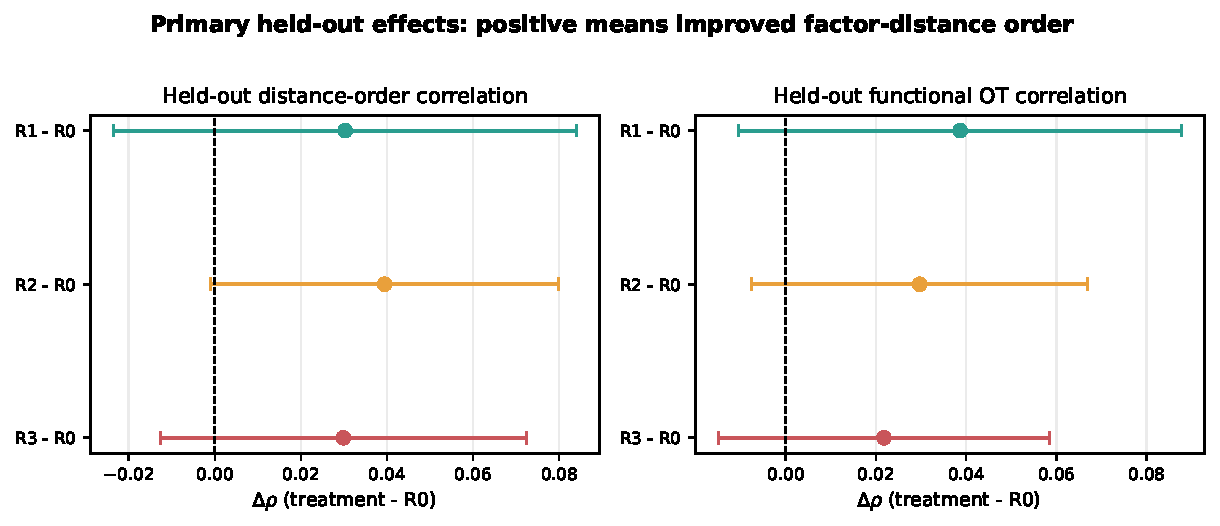
\includegraphics[width=.88\textwidth]{figures/heldout_effect_forest.pdf}\caption{v1.1.1 held-out effects motivating the repair. Positive means for R3 were not seed-robust.}\end{figure}
\begin{figure}[H]\centering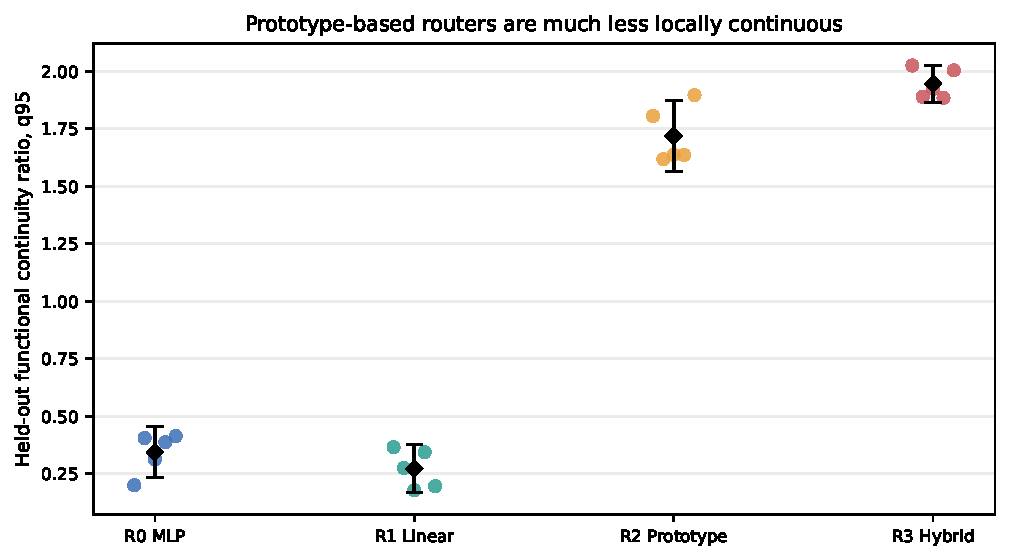
\includegraphics[width=.82\textwidth]{figures/continuity_q95.pdf}\caption{v1.1.1 functional q95 continuity. Prototype-dominated routes were markedly sharper than R0/R1.}\end{figure}
\section{Isolation retained from v1.1.1}
For every seed, the experiment freezes
\[
P^\star,\quad C_\phi^\star,\quad \{g_h^\star\}_{h=1}^H,\quad Q^\star,\quad C^\star.
\]
Only the router is trained. This preserves the causal interpretation
\[
\text{factor}\rightarrow c\rightarrow r\rightarrow\text{fixed host functions}.
\]
\begin{figure}[H]\centering
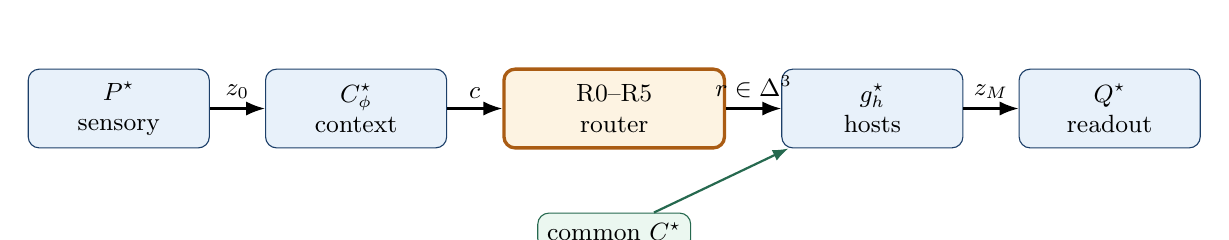
\begin{tikzpicture}[node distance=7mm and 7mm,every node/.style={font=\small,align=center},frozen/.style={draw=deepblue,fill=softblue,rounded corners,minimum width=23mm,minimum height=10mm},train/.style={draw=deeporange,fill=softorange,rounded corners,very thick,minimum width=28mm,minimum height=10mm},arrow/.style={-{Latex[length=2.4mm]},thick}]
\node[frozen] (p) {$P^\star$\\sensory};\node[frozen,right=of p] (c) {$C_\phi^\star$\\context};\node[train,right=of c] (r) {R0--R5\\router};\node[frozen,right=of r] (h) {$g_h^\star$\\hosts};\node[frozen,right=of h] (q) {$Q^\star$\\readout};
\draw[arrow](p)--node[above]{$z_0$}(c);\draw[arrow](c)--node[above]{$c$}(r);\draw[arrow](r)--node[above]{$r\in\Delta^3$}(h);\draw[arrow](h)--node[above]{$z_M$}(q);
\node[below=8mm of r,draw=deepgreen,fill=softgreen,rounded corners] (cost) {common $C^\star$};\draw[-{Latex[length=2mm]},deepgreen,thick](cost)--(h);
\end{tikzpicture}
\caption{v1.1.2 keeps the successful bridge-isolation protocol.}
\end{figure}
\section{Smooth simplex-residual router}
The base logits are linear:
\[
\ell^{\mathrm{base}}(c)=Wc+b.
\]
Prototype scores are centered and standardized across hosts, then bounded:
\[
\delta_h(c)=\tanh\!\left(\frac{s_h(c)-\overline s(c)}{\operatorname{Std}_k s_k(c)+\varepsilon}\right).
\]
A scalar context gate controls their amplitude:
\[
g(c)=\sigma(u^\top\phi(c)+\beta),\qquad 0\le g(c)\le 1.
\]
The final route is
\[
\ell_h(c)=w_h^\top c+b_h+s_{\max}g(c)\delta_h(c),\qquad r(c)=\operatorname{softmax}(\ell(c)/\tau),
\]
with preregistered $s_{\max}=0.35$. The global linear channel cannot be erased by a local prototype term, and the residual cannot exceed the cap.
\subsection{Context-only continuity hinge}
R5 adds
\[
\loss_{\mathrm{cont}}=\E_{a<b}\left[\max\bigl(0,d_R(r_a,r_b)-\kappa d_C(c_a,c_b)-m\bigr)^2\right].
\]
This loss uses inferred contexts and route-simplex distances only. It does not use rotation labels. R4 and R5 separate architecture from regularization.
\section{Covariance and SPD diagnostic axis}
For each dense factor value $u$, contexts across source identities define
\[
\Sigma_u=(1-\lambda)\widehat{\operatorname{Cov}}(c\mid u)+\lambda\frac{\operatorname{tr}(\widehat\Sigma_u)}{d}I+\epsilon I.
\]
The diagnostic compares
\begin{align}
d_{\mathrm{LE}}(\Sigma_u,\Sigma_v)&=\norm{\log\Sigma_u-\log\Sigma_v}_F,\\
d_{\mathrm{AIRM}}(\Sigma_u,\Sigma_v)&=\norm{\log(\Sigma_u^{-1/2}\Sigma_v\Sigma_u^{-1/2})}_F,
\end{align}
and Bures-Wasserstein distance. A combined metric adds normalized centroid and covariance distances. Passing this diagnostic would mean covariance adds measurable factor information; it would not prove a learned Riemannian manifold.
\section{Treatments and ablations}
\begin{table}[H]\centering\small\begin{tabularx}{\textwidth}{@{}lXl@{}}\toprule
Method & Definition & Role\\\midrule
R0 & flexible MLP & operational baseline\\
R1 & linear context router & smooth low-capacity reference\\
R2 & prototype energy & local-territory reference\\
R3 & directional-prototype hybrid & failed v1.1.1 treatment\\
R4 & bounded smooth residual & architecture repair\\
R5 & R4 plus context-only continuity & primary treatment\\\bottomrule
\end{tabularx}\end{table}
All methods receive identical forward-image and optimizer-step budgets. No angle-supervised route loss is used.
\section{Metrics and preregistered gates}
The common-cost functional route distance remains entropic optimal transport:
\[
W_{C^\star}^{\varepsilon}(r_a,r_b)=\min_{\Pi\mathbf 1=r_a,\Pi^\top\mathbf 1=r_b}\langle\Pi,C^\star\rangle+\varepsilon\operatorname{KL}(\Pi\Vert r_ar_b^\top).
\]
Primary gates are:
\begin{enumerate}[leftmargin=1.8em]
\item R5--R1 held-out functional stress has an upper seed bound below zero and at least four favorable seeds.
\item R5--R1 held-out functional $\rho$ has a lower seed bound above zero and at least four favorable seeds.
\item R5 functional q95 continuity is not more than 0.10 above R1 at the upper seed bound.
\item Far route swaps exceed near swaps in at least four of five seeds.
\item Functional CSR and prediction-identity gates pass.
\item R5 remains within the one-point operational margin versus R0.
\item Combined centroid-plus-SPD stress improves over centroid-only with an upper seed bound below zero.
\end{enumerate}
\section{Required evidence and verification}
The notebook exports per-seed and aggregate route geometry, continuity distributions, route swaps, mediation probes, causal interventions, allocation territories, accuracy/forgetting, regularized covariance matrices, pairwise SPD distances, gate tables, corrected manifests, and environment capture. The independent Verification Stack consumes the execution PDF and ZIP and emits metric, protocol, claim, evidence-bundle, and summary files.
\section{Non-claims and next stages}
\begin{claimbox}[Epistemic boundary]
v1.1.2 does not claim operational superiority, mature host specialization, memory transport, full Energy-Guided control, reinforcement-learning control, a learned Riemannian manifold, or quantum advantage.
\end{claimbox}
If the smooth residual treatment qualifies, v1.1.3 will study route-function memory distributions and transport. v1.1.4 will then reintroduce selective host plasticity, contribution-weighted ablations, recovery, and cross-seed specialization. Explicit host-to-router feedback remains a G2.1 stage, while TPUT adds goal-conditioned future control.
\section{Conclusion}
Version 1.1.2 is an evidence-driven repair, not a geometric escalation for its own sake. It preserves the valid isolation design of v1.1.1, bounds the prototype contribution, controls continuity without external factor labels, and treats SPD covariance geometry as a diagnostic that must earn its place through measurable improvement.
\end{document}
